\chapter{Resultados e Discussão}
\label{cap:resultados}

Este capítulo discute os resultados obtidos ao longo do desenvolvimento do sistema automatizado de limpeza e manutenção de piscinas. São analisados desempenho o da solução proposta, desafios técnicos enfrentados durante a implementação e as estratégias adotadas para mitigá-los. A discussão contempla integração do protótipo físico, usabilidade da interface de controle desenvolvida e confiabilidade dos dados coletados, destacando os avanços alcançados em relação aos métodos manuais tradicionais, bem como limitações observadas no contexto experimental.

\section{Integração do Protótipo Físico}

O desenvolvimento do protótipo físico possibilitou a consolidação da arquitetura definida na fase de Elaboração, permitindo validar, de forma prática, a integração entre sensores, atuadores e central de controle. O conjunto foi acondicionado em uma caixa de papelão coberta por placa de isopor com o objetivo de simular ambiente real de operação e prover proteção aos componentes eletrônicos contra respingos e umidade, características inerentes ao contexto de uso em piscinas.

A disposição dos sensores de pH, turbidez, temperatura e nível no reservatório de testes mostrou-se adequada para a realização de leituras contínuas, contribuindo para obtenção de dados consistentes ao longo dos experimentos. Essa configuração evidenciou confiabilidade na coleta das variáveis monitoradas, aspecto essencial para o funcionamento correto do ciclo de automação proposto.

A Figura \ref{fig:prototipo_final} apresenta visão geral do protótipo, destacando a interligação entre central de controle e dispositivos responsáveis pela medição e atuação no sistema.

\begin{figure}[H]
    \centering
    \caption{Protótipo final do sistema de automação.}
    \label{fig:prototipo_final}
    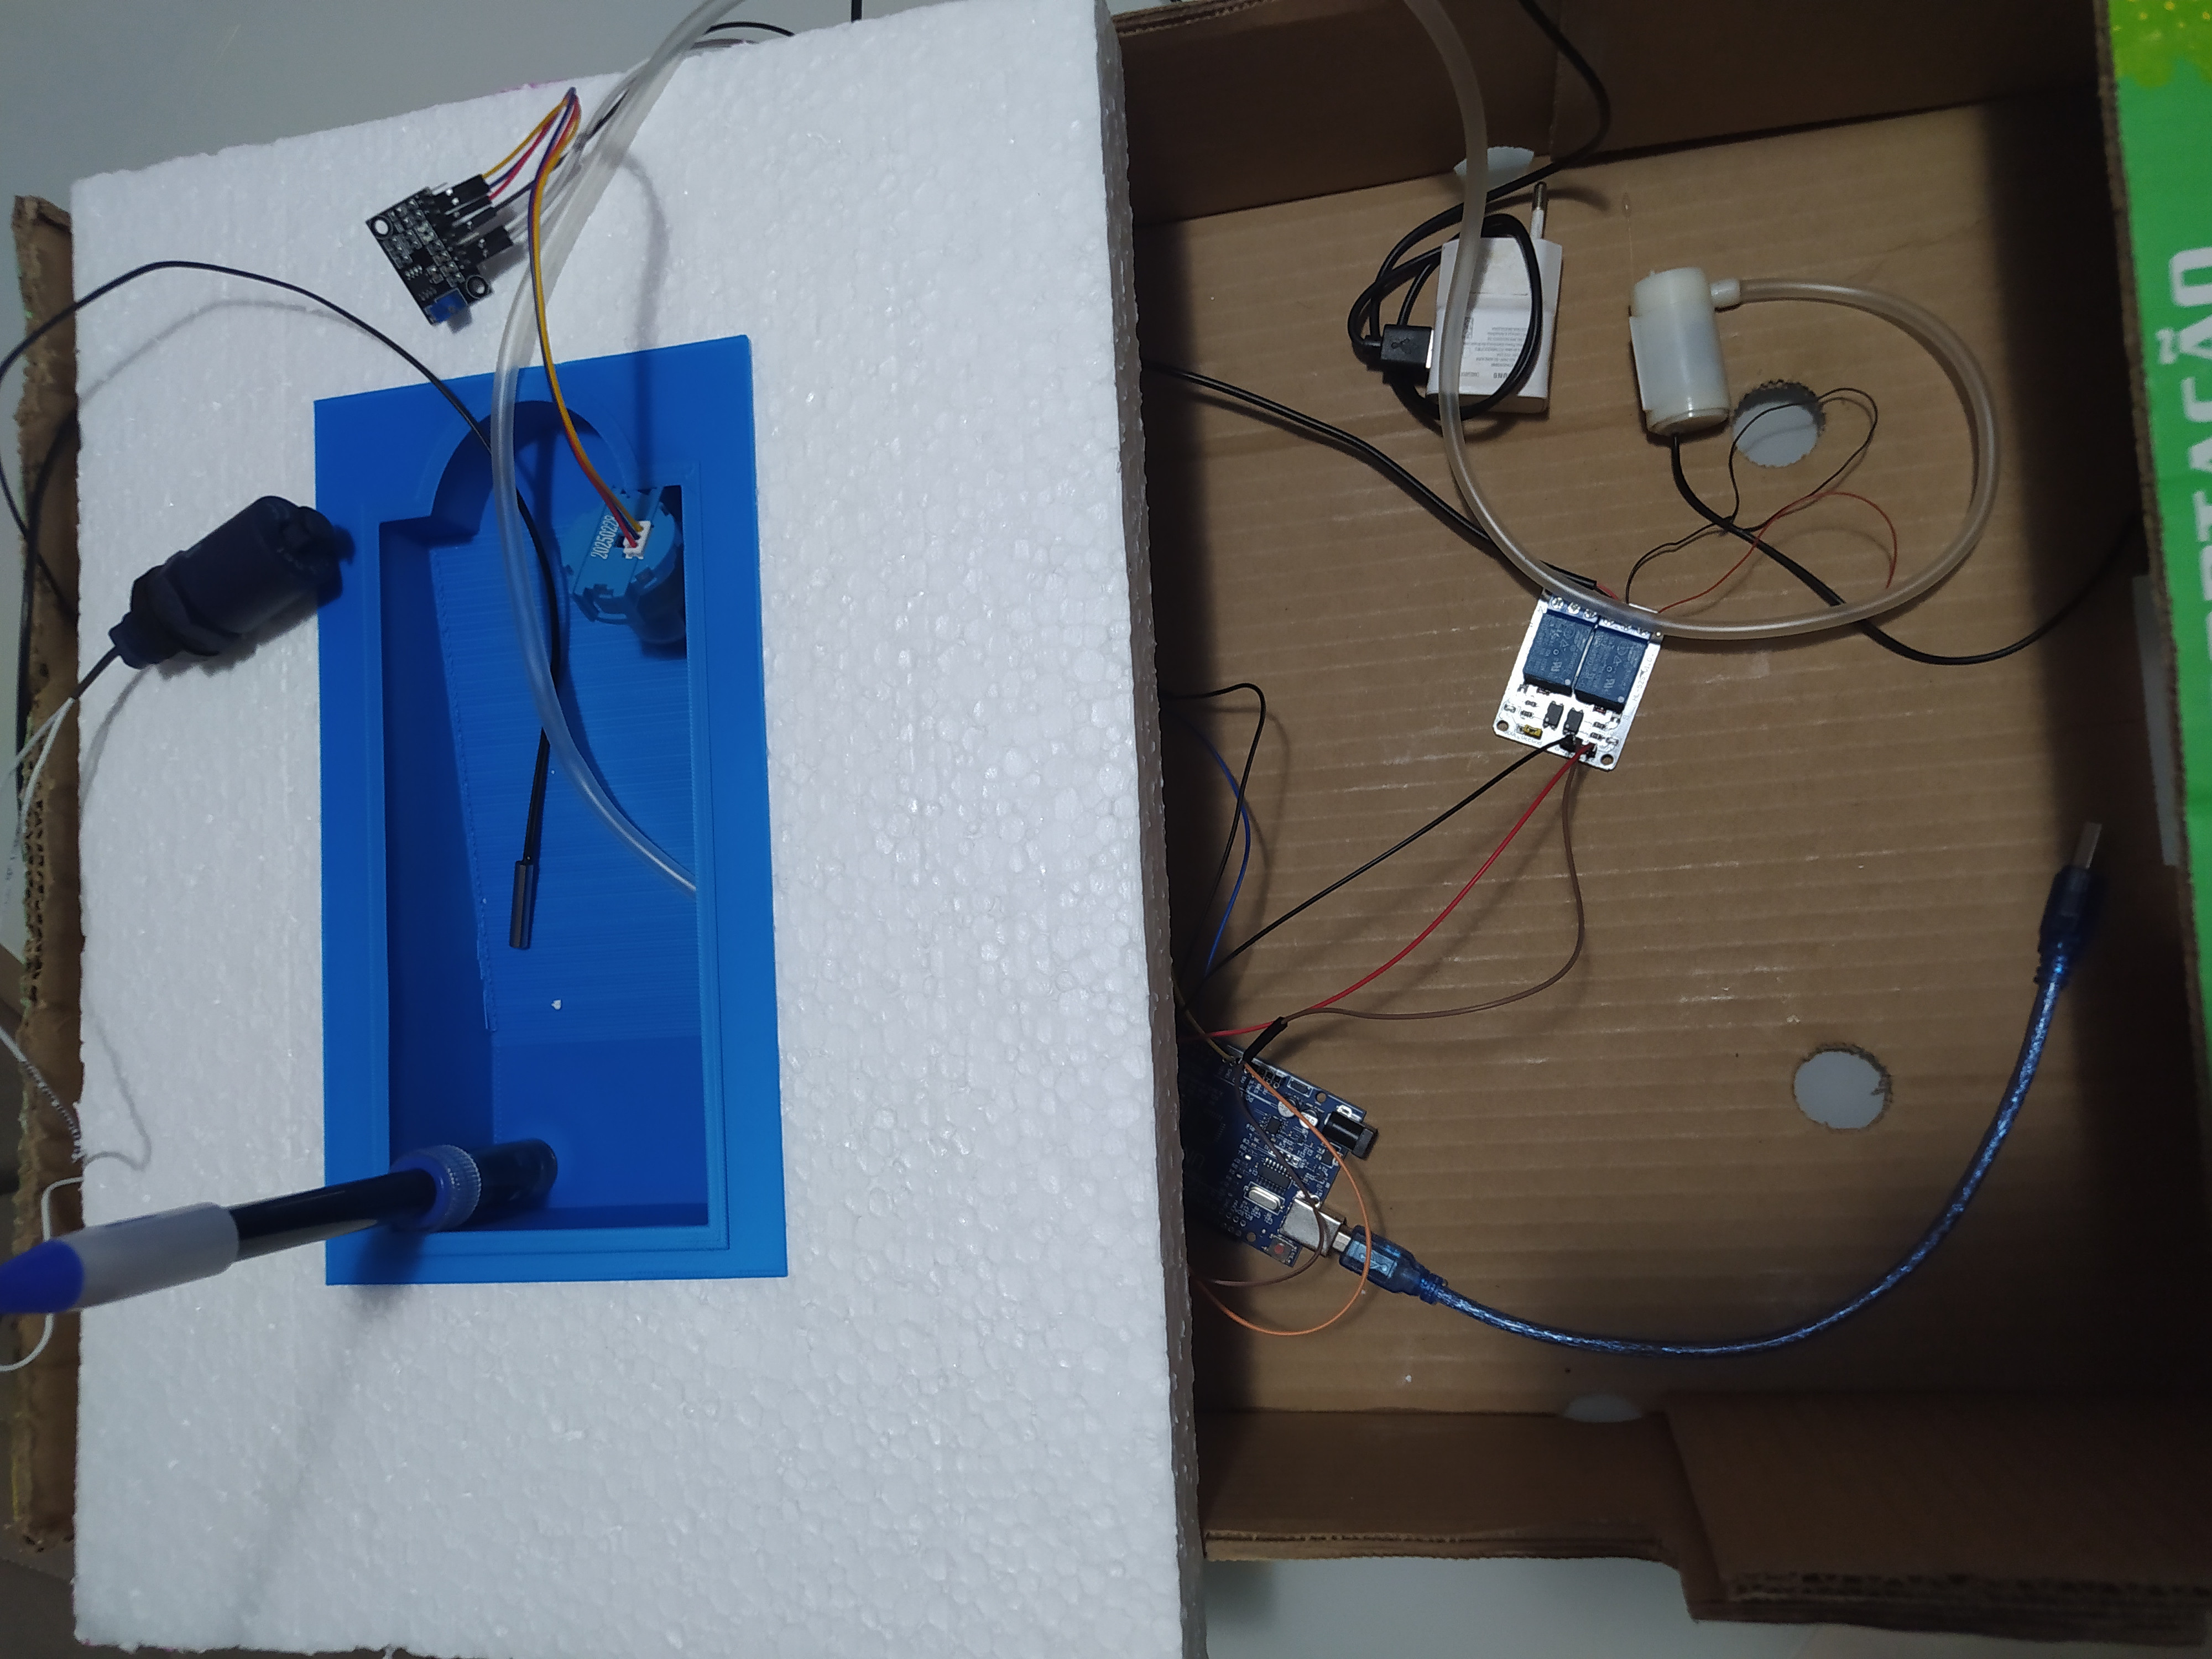
\includegraphics[width=0.8\textwidth]{imagens/prototipoFinal.jpg}
    \caption*{Fonte: Autoria própria (2025).}
\end{figure}

Durante os testes de integração, o conjunto de atuadores apresentou comportamento compatível com o esperado, com acionamento da bomba d’água por meio do relé ocorrendo de forma quase imediata. Entretanto, nas etapas iniciais de validação, foi identificado um problema relacionado à estabilidade do sistema: o acionamento da bomba gerava ruídos eletromagnéticos e picos de tensão que interferiam no funcionamento do microcontrolador, comprometendo a estabilidade das leituras dos sensores e a operação contínua do atuador.

Para mitigar esse problema, optou-se pela substituição do módulo de acionamento simples por módulo relé com isolamento por optoacoplador\footnote{Um componente eletrônico que transfere sinais elétricos entre dois circuitos isolados galvanicamente, utilizando luz para evitar interferências e proteger componentes sensíveis}. Essa solução proporcionou o isolamento galvânico\footnote{Separação física e elétrica entre dois ou mais circuitos, impedindo o fluxo direto de corrente contínua (CC) entre eles, enquanto permite a transferência de sinal ou potência} entre o circuito de potência e circuito lógico do \textit{Arduino}, eliminando interferências e aumentando a robustez do sistema. A Figura \ref{fig:rele_opto} apresenta o componente adotado após essa modificação.

\begin{figure}[H]
    \centering
    \caption{Relé com optoacoplador.}
    \label{fig:rele_opto}
    \includegraphics[width=0.60\textwidth]{imagens/releFinal.jpeg}
    \caption*{Fonte: Autoria própria (2025).}
\end{figure}

Além das questões relacionadas ao acionamento dos atuadores, foram identificadas limitações associadas à calibração de alguns sensores. O sensor de pH, apresentou descalibração de fábrica, exigindo ajuste manual no módulo ao qual estava acoplado. A calibração foi realizada em nível de \textit{hardware}, por meio do ajuste do potenciômetro (\textit{trimpot}) de \textit{offset}\footnote{um pequeno potenciômetro de precisão montado diretamente em uma placa de circuito (PCB) para calibração, focado em zerar tensões indesejadas (offset) ou ajustar níveis de sinal} da placa condicionadora, alinhando tensão de saída e valor de referência esperado.

O procedimento de calibração foi validado utilizando-se água mineral, cujo pH declarado é de 6,98. Após o ajuste, o sensor apresentou leituras variando entre 6,78 e 6,80, consideradas satisfatórias para o contexto experimental, conforme ilustrado na Figura \ref{fig:sensorpH:sendoCalibrado}.

\begin{figure}[H]
    \centering
    \caption{Validação do sensor de pH.}
    \label{fig:sensorpH:sendoCalibrado}
    \includegraphics[width=1.00\textwidth]{imagens/calibracaoSensorPh.png}
    \caption*{Fonte: Autoria própria (2025).}
\end{figure}

O sensor de temperatura apresentou desvios em relação ao valor de temperatura real da água. A correção foi realizada via \textit{software}, por meio da aplicação de fator de ajuste na equação do divisor de tensão, compensando variações na resistência nominal do termistor\footnote{Um tipo de resistor semicondutor cuja resistência elétrica varia significativamente com a temperatura} do tipo NTC. A validação do ajuste foi conduzida com base na comparação entre a leitura fornecida por um termômetro de piscina e os valores obtidos pelo sensor, registrando-se 25,7~°C no instrumento de referência e 25,93~°C no sistema desenvolvido. Essa proximidade entre valores confirma a adequação do processo de calibração, conforme apresentado na Figura \ref{fig:sensorTemperatura:sendoCalibrado}.

\begin{figure}[H]
    \centering
    \caption{Validação do sensor de temperatura.}
    \label{fig:sensorTemperatura:sendoCalibrado}
    \includegraphics[width=1.00\textwidth]{imagens/calibrandoSesorTemperatura.png}
    \caption*{Fonte: Autoria própria (2025).}
\end{figure}

\section{Interface de Controle e Monitoramento}

A interface de controle desenvolvida, implementada no \textit{front-end} com a biblioteca \textit{React}, foi projetada com objetivo de centralizar informações técnicas em um \textit{dashboard} visualmente intuitivo. Essa abordagem busca abstrair a complexidade inerente aos sensores e processamento dos dados, permitindo que o usuário compreenda rapidamente o estado da piscina sem necessidade de conhecimentos técnicos avançados.

Diferentemente de soluções que exigem interpretação direta de valores ou interação por meio de \textit{displays LCD} acoplados ao \textit{hardware}, a interface \textit{web} apresenta os principais indicadores de qualidade da água de forma gráfica e organizada. Ao acessar o sistema, o usuário visualiza, em tempo real, cartões de \textit{status} referentes aos parâmetros monitorados, como pH, temperatura, turbidez e estado da bomba.

A comunicação entre \textit{front-end} e \textit{back-end}, desenvolvido em \textit{Spring Boot}, garante atualização periódica dos dados exibidos, permitindo acompanhamento contínuo da evolução do tratamento da água. Além do monitoramento passivo, a interface oferece recursos de controle ativo, possibilitando ao usuário ligar ou desligar manualmente o sistema de filtragem. Essa funcionalidade permite sobreposição temporária da lógica de automação em situações específicas, como manutenções corretivas ou testes operacionais.

A Figura \ref{fig:dashboard_web} apresenta a tela principal do sistema, evidenciando a disposição dos indicadores e o foco na clareza das informações exibidas.

\begin{figure}[H]
    \centering
    \caption{Interface \textit{Web}: Dashboard de monitoramento em tempo real.}
    \label{fig:dashboard_web}
    \includegraphics[width=1.0\textwidth]{imagens/printSistema.png}
    \caption*{Fonte: Autoria própria (2025).}
\end{figure}

\vspace{5em}

\section{Análise de Desempenho e Discussão}

Os testes práticos realizados no cenário de validação demonstraram que o sistema é capaz de executar de forma consistente o ciclo completo de automação proposto, abrangendo etapas de leitura dos sensores, processamento dos dados, transmissão das informações e atuação sobre dispositivos físicos. Essa integração confirmou a viabilidade da arquitetura adotada para aplicações de automação residencial em piscinas.

No que se refere à precisão das medições, o sensor de temperatura NTC 10K apresentou estabilidade, com variações reduzidas quando comparadas às leituras obtidas por meio de termômetro de referência. Esse comportamento evidencia a adequação do componente para monitoramento térmico contínuo em ambientes domésticos. Em contrapartida, os sensores analógicos voltados à avaliação da qualidade da água demandaram tratamento mais cuidadoso, tanto em nível de \textit{hardware} quanto de \textit{software}.

Durante testes iniciais, observou-se que, na ausência de técnicas de filtragem digital, as leituras de pH e turbidez apresentavam oscilações momentâneas decorrentes de ruídos elétricos e variações ambientais. Essas flutuações poderiam ocasionar acionamentos indevidos da bomba, comprometendo a eficiência do sistema e aumentando o desgaste dos componentes. Para mitigar esse comportamento, foram implementados filtros de média móvel no \textit{firmware} do \textit{Arduino}, estratégia que reduziu significativamente o ruído nas leituras e proporcionou estabilidade ao processo decisório. Após essa intervenção, o sistema apresentou desempenho compatível com os requisitos de uso doméstico, mantendo respostas coerentes com as condições reais da água.

Outro aspecto relevante avaliado foi a latência de comunicação, definida como um dos requisitos não funcionais críticos do sistema. Os experimentos indicaram que o tempo médio entre detecção de evento físico (como identificação de nível inadequado de água) e atualização correspondente na interface \textit{web} permaneceu, na maioria dos testes, abaixo de cinco segundos. Esse resultado valida a eficiência da arquitetura distribuída baseada em \textit{API REST} e demonstra que a solução atende demandas típicas de aplicações IoT residenciais, nas quais resposta em tempo quase real é suficiente para garantir segurança e confiabilidade operacional.

Algumas limitações foram identificadas. Destacam-se a sensibilidade dos sensores analógicos de baixo custo, suscetíveis a ruídos e variações ambientais, e a dependência da estabilidade da rede \textit{Wi-Fi} local, fator que pode impactar a atualização contínua da interface em cenários com conectividade limitada. Tais restrições não comprometem a funcionalidade do protótipo, mas indicam necessidade de aprimoramentos para aplicações em maior escala ou ambientes com exigências mais rigorosas. Esses aspectos orientam propostas de evolução do sistema, discutidas na seção de trabalhos futuros.

\section{Trabalhos futuros}

Como continuidade deste trabalho, diversas possibilidades de aprimoramento podem ser exploradas a fim de ampliar a robustez, autonomia e escalabilidade do sistema desenvolvido. Uma evolução natural consiste na integração de sensor de cloro livre, baseado em potencial de oxirredução (ORP), permitindo completar o ciclo de automação química da piscina e oferecer controle mais preciso da desinfecção da água.

Outra linha refere-se à aplicação de algoritmos de aprendizado de máquina voltados à manutenção preditiva. A partir do histórico armazenado no sistema, seria possível identificar padrões de funcionamento e antecipar falhas em bombas, sensores ou outros componentes, reduzindo custos de manutenção e aumentando a confiabilidade da solução.

Adicionalmente, recomenda-se implementação do sistema em piscinas de alvenaria em escala real, possibilitando avaliação do desempenho em condições próximas do uso cotidiano. Esse cenário permitiria analisar o comportamento do sistema sob diferentes volumes de água, condições ambientais e perfis de utilização, contribuindo para a validação de sua aplicabilidade e eventuais ajustes de projeto.

No que diz respeito à escalabilidade, futuras versões do sistema podem incorporar suporte a múltiplas piscinas e usuários simultâneos, ampliando seu escopo de aplicação para condomínios, clubes ou empreendimentos de lazer. Para sustentar essa expansão, propõe-se adoção de arquitetura orientada a eventos no \textit{back-end}, utilizando o padrão de projeto \textit{Observer}. Essa abordagem permitiria que a interface \textit{web} fosse notificada de forma proativa e instantânea sempre que novas leituras fossem processadas, eliminando a necessidade de requisições cíclicas (\textit{polling})\footnote{Técnica na qual um sistema realiza verificações periódicas em intervalos regulares para identificar a ocorrência de novos dados ou eventos.}. Como resultado, espera-se redução no consumo de recursos computacionais, eficiência na comunicação e experiência de uso mais fluida para o usuário final.


    